\chapter{Introduction}\label{chapter:introduction}

\section{The Setting}
\subsection{Let there be Bitcoin}
Before money, there was debt~\cite{debt}. Money is a yardstick for measuring
it. Sometimes it takes the form of a gold coin. Not useful in itself, one
accepts it because one assumes other people will. Modern \emph{fiat} money is
not backed by gold, but takes the form of pieces of paper bills or, more often,
bits in the computer systems of banks. Regardless of their manifestation, all
forms of money are debt, which is a social relation~\cite{critical-realism}.

Money functions as a \emph{medium of exchange}, as a \emph{common measure of
value} or \emph{unit of account}, as a \emph{standard of value} or
\emph{standard of deferred payment}, and a \emph{store of
value}~\cite{money-mechanism}. These functions of money rely on the relationship
of the individual with the economic community that accepts money. Each monetary
transaction between two parties is never a ``private matter'' between them,
because it translates to a claim upon society~\cite{philosophy-of-money}.

This gives rise to the need of \emph{consensus}. The economic community must be
able to ascertain, in principle, whether a monetary transaction is \emph{valid}
according to its rules. In a good monetary system, parties of the economic
community must globally agree on the conclusions of such deductions. In simple
words, when someone pays me, I must know that they have sufficient money to do
so, and that this money given to me will be accepted by the economic community
when I later decide to spend it. This judgement of validity consists of two
parts: First, that the money in use has been minted legitimately in the first
place. Secondly, that this money rightfully belongs to the party who is about to
spend it, and has not been spent before, to protect against \emph{double spending}.

The problem of consensus is solved differently in different monetary systems. Gold
coins had stamps whose veracity could be checked, while paper bills have chemical
features making them difficult to duplicate. Such physical features ensure the
legitimacy of minting. The problem of double spending is trivial when it comes to
physical matter: If I give a
gold coin to someone, I no longer hold that gold coin and cannot also give it to
someone else. When coins are digitized, the problem of \emph{who owns what}
is solved by the private bank and payment processors.
A private bank centrally maintains the balance of a bank account to ensure a
corresponding debit card cannot spend more money than it has. In this case, a
vendor's terminal connects to the bank's servers to check the validity of the
payment (and security can only be ensured while the terminal is online). These
cases involve a \emph{trusted third party}\index{Trusted Third Party}, the
bank or the payment processor, to maintain a balance and make a judgement on
whether a transaction is valid. The central bank is relied upon for the
legitimacy of minting. Payment processors and banks who maintain account
balances and make a judgement on whether a transaction is valid are relied upon
to prevent double spending. The economic community depends on these third
parties and trusts them for availability and truthfulness.

The cypherpunk\index{Cypherpunks} political movement and the wave of
cryptographers working on \emph{protocols} in general have an inherent hatred
for trusted third parties. For the former, they amount to
centralization of political power which they wish to see eliminated. For the
latter, it constitutes a technical challenge -- if the role of the trusted
third party is fully algorithmizable, why not replace the party by a protocol
ran by the economic community themselves? It is somewhere in the intersection of the
two that \emph{blockchain} protocols appeared.

Bitcoin\index{Bitcoin} was invented by Satoshi Nakamoto\index{Satoshi Nakamoto}
in 2008. In a paper titled
\emph{A Peer-to-Peer Electronic Cash System}~\cite{bitcoin}, Satoshi introduced
the first \emph{cryptocurrency} and the technology powering it, the
\emph{blockchain}. The paper accompanied an implementation of what has come to
be known as \emph{Bitcoin Core}\index{Bitcoin Core}, the first cryptocurrency
wallet. Satoshi, whose name was soon deified within
the blockchain community, was nothing but a Japanese pseudonym, the
physical identity and whereabouts of the author or authors still unknown. Never
short on drama, the space was shaken again when Satoshi mysteriously disappeared
without a trace in 2011, leaving the community leaderless, perhaps in an attempt
to, in a sense, remove the last standing trusted third party from the picture.

As an electronic currency, Bitcoin enjoys many advantages. The transfer of
a transaction takes a couple of seconds, while transactions become secure
against chargebacks in about an hour. It is easy and cheap to move money across
the world in large quantities, with transaction fees remaining constant
regardless of amount moved (at the time of writing, approximately $\$0.05$). The
ecosystem is open, the reference client open source, and the community can
develop their own software to work with it without requesting permission from
anyone.

More interestingly, Bitcoin is the first \emph{decentralized} electronic
currency. Unlike all previous electronic currencies, it does not require any
trusted third party for its operation. There is no company or operator with
privileged access over Bitcoin -- no CEO or corporate network. This makes
the Bitcoin network \emph{sovereign}: It cannot be shut down by a traditional
court of law regardless of the desires of world governments, unless drastic
measures are employed such as shutting down the Internet. There is no central
entity to issue a subpoena to and it will continue to operate as long as there
are users. This also makes the system uncensorable.

\subsection{Coming to an agreement}
Bitcoin is a peer-to-peer network. As such there are no servers and clients.
Instead, similar to BitTorrent, there are simply nodes which connect to each
other and exchange data. These form the global Bitcoin network, a connected
graph of participants continuously exchanging financial data. They run open
source code which can be inspected and modified by anyone, and are all
treated as equals, none of them enjoying elevated privileges. Additionally, there
is no implicit trust. It is accepted that some of them will behave adversarially
and try to subvert the system by attempting to spend money they do not own,
or by attempting to censor others.

At first glance, given that anyone can modify the code of their node, it seems
that the situation is hopeless. Is it not possible for such a node to fake how
much money they have? Additionally, even if they cannot conjure money out of
nowhere, since money is represented as bits, is it not possible to simply
duplicate their wallet and thus duplicate their money? In this setting, the
consensus problem now becomes critical and particularly challenging. Bitcoin
resolves such issues by making use of the \emph{blockchain}.
Bitcoin's security, and in turn our analysis, is for \emph{arbitrary
adversaries}. The powerful cryptographic setting gives us the tools not only to
analyze particular adversarial strategies, but to prove our system can withstand
\emph{any} adversary, even ones we cannot imagine. As such, our security
theorems will begin ``For any adversary...''

To solve the consensus problem, Bitcoin makes a radical shift compared to
previous systems. To allow participants to verify whether a transaction is valid
and whether the payer has sufficient money to execute it, it reveals to
\emph{all}
participants who owns how much money. This is done by dissemminating all
transactions to all participants in the network in a gossiping fashion. These
transactions are then stored by \emph{every} other node in perpetuity. Any
synchronizing node downloads these historical transactions and stores them, too.
By looking at these transactions, it can deduce whether a party's claim to spend
money is legitimate. The financial privacy of the parties is not trivially
violated, because money is received into \emph{public keys} instead of accounts
corresponding to real names. Privacy can be significantly improved when a person
employs a new public key for every transaction they are about to
receive~\cite{bitcoin-dev-guide}.

A transaction in Bitcoin is a payment order in the form of a string. It has a
source, which corresponds to a previous transaction receiving the money, and a
destination, which is a public key. In order for a transaction to be valid, the
private key corresponding to the public key in the source must digitally sign the
transaction, including the public key of the new owner. If Alice wishes to pay
Bob, she looks for a transaction which has paid her money that she has not yet
spent. She then creates a payment order in which she writes down the amount she
wishes to pay to Bob, as well as his public key, and signs the order with her
private key. She then broadcasts this transaction on the peer-to-peer network.
Bob, who is connected to the same network, receives the transaction through one
of his peers, and verifies its validity as well as the fact that his own public
key has been used in the payment and that the amount is correct.

Each node organizes the transactions it sees on the network into a
\emph{ledger}, which is a sequence of transactions. This ledger determines which
party has how much money. The node can then evaluate the validity of a new
incoming transaction by assessing whether there are sufficient funds. For the
monetary system to function, the parties must globally agree on a \emph{common}
ledger. If Alice receives a payment from Bob and her ledger depicts this, but
Charlie's does not, then Alice's money received from Bob cannot be used to pay
Charlie.

A malicious node can attempt to \emph{double spend}. If Eve legitimately owns a
coin, she can create a valid transaction $\tx$ paying Alice with that coin, as
well as a valid transaction $\tx'$ paying Bob with that coin. If any of the two
transactions are individually broadcast on the network, it will be considered
valid. However, if both transactions are broadcast on the network, they cannot
both be valid, because Eve only ever had one coin. As such, a strategy against
double spending must be employed when such a sitatuation occurs.

Simple strategies do not work. For example, observing that Eve must be malicious
to have created a double spend, the nodes could reject \emph{both} of her
transactions. However, this now enables Eve to first pay Alice for some service,
but later invalidate that payment by also paying Bob. While Eve cannot profit
from this, she can harm Alice. The alternative strategy of waiting a fixed time
$\Delta$ to determine whether there have been any double spends prior to
accepting a transaction also does not work. The reason is that Eve could
broadcast her double spending transaction at a time just before $\Delta$ has
elapsed. Because the network is not fully synchronized, some parties will
receive the transaction prior to time $\Delta$, while others will receive it
after time $\Delta$, causing the network to disagree about whether the first
transaction is valid.

\subsection{Chains of blocks}
To solve this problem, nodes must place transactions in chronological order. As
Eve can lie about the timestamps of her transactions or broadcast them at a
delayed time, timestamps cannot be trusted.

Transactions on the network are collected by nodes into bundles called
\emph{candidate blocks}. These blocks are simply strings concatenating the
transactions together with some metadata. The nodes that collect them are known
as \emph{miners} and anyone can participate as a miner. Each miner attempts to
\emph{mine} the candidate block it has created, turning it into a \emph{block}.
Mining involves solving a moderately hard problem and has a small, but not
negligible, probability of success. When the problem is successfully solved, we
say that a block has been \emph{found} or \emph{mined}. The block contains the
transactions, metadata, as well as the solution to the moderately hard problem.
The moderate hardness of mining ensures blocks are created at a predetermined
expected rate. For Bitcoin, this rate is $10$ minutes. Once a block is found, it
is broadcast to the rest of the network. A transaction is considered
\emph{confirmed} once it has been included in a block. Transactions inside
blocks are placed in an arbitrary order determined by the party creating the
block. Block validity mandates that no double spends appear within the same
block. Once a transaction is confirmed in a block, it is considered to have been
placed in order among other transactions.

A block includes a pointer to the most recent block seen by the node. This
creates a \emph{chain of blocks} or \emph{blockchain}. As each block contains
transactions, reading the transactions within the blockchain in order gives a
unique ledger signifying which transaction happened before which other
transaction. The validity of the blockchain requires that the transactions in
the new block do not conflict with transactions in the previous chain, and so
reading the transaction sequence of a valid blockchain always gives a valid
transaction sequence. Whenever a node receives a blockchain from the
network, if it is longer than its own blockchain in the number of blocks it
contains, then it abandons its own blockchain and adopts the longer one. This is
known as the \emph{longest chain rule}. The first block of the blockchain,
called the \emph{genesis} block, was fixed by the protocol at the time of
initial deployment.

\begin{figure}[h]
    \caption{
    A blockchain with some temporary forks. Squares depict blocks.
    }
    \centering
    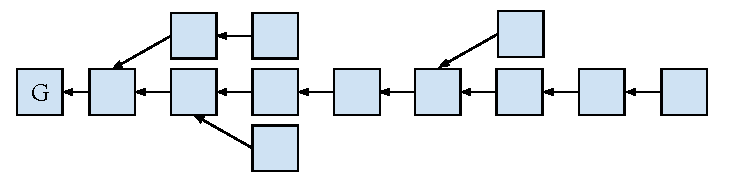
\includegraphics[width=0.7\columnwidth,keepaspectratio]{chapters/introduction/figures/blockchain.pdf}
    \label{fig.blockchain}
\end{figure}

Surprisingly, this simple rule solves the consensus problem. Because blocks are
broadcast once every $10$ minutes on average, this leaves a sufficient window of
silence between blocks so that honest parties will adopt the same chain. If it
happens that two blocks are found almost simultaneously by chance, some parties
will mine on top of one chain, while others will mine on top of another. Once a
new block is found, one of the two chains will grow longer and the population
will migrate to the longest chain, abandoning the shorter chain and reaching
consensus. These are known as \emph{temporary forks}\index{Temporary Fork}. The
chance of two blocks being found simultaneously again and again is small, and
hence eventually the network will converge to a common view. This is illustrated
in Figure~\ref{fig.blockchain}. The honest parties may have some small
disagreement about which few blocks are at the end of the blockchain. However,
they will share a large \emph{common prefix}. As such, a transaction is
considered safe once it has been buried under a sufficient number of blocks.

Once a transaction $\tx$ is confirmed by becoming included in some block $b$ and
that block is buried under a sufficiently large number of blocks, it
becomes difficult for the adversary to double spend using a conflicting
transaction $\tx'$. Consider the execution in Figure~\ref{fig.adversary-race}.
As blockchains extending $b$ do not validate if they
contain $\tx'$, the adversary must \emph{fork} the blockchain and start mining
on top of the parent of $b$. Consider the first block $b'$ of that fork in which
$\tx'$ is confirmed. This becomes a mining race between the honest parties, who
are mining on top of the longest chain extending $b$ and confirming $\tx$, and
the adversary who is mining a new chain on top of $b'$ and confirming $\tx'$. If
we assume the honest parties control the majority of the computational power on
the network, the chain that the honest parties mine will grow faster than the
one extended by the adversary. This is known as the \emph{honest majority
assumption}.

\begin{figure}[h]
    \caption{
    A minority adversary fails to double spend a deeply burried transaction.
    }
    \centering
    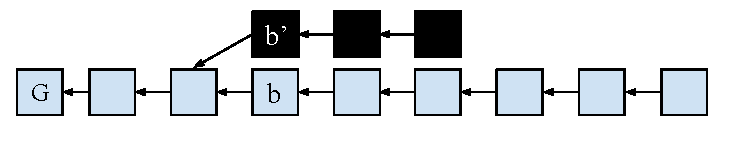
\includegraphics[width=0.7\columnwidth,keepaspectratio]{chapters/introduction/figures/adversary-race.pdf}
    \label{fig.adversary-race}
\end{figure}

When a miner is asked to find a block, they collect the unconfirmed transactions
into a string $\overline{x}$. They then attempt to find a $\textsf{nonce}$ such
that $H(\overline{x} \concat \textsf{nonce} \concat h') \leq T$, where $T$ is a constant
\emph{target}, $H$ is a cryptographically secure hash function, and $h'$ is the
hash of the previous block. As the hash
function has an unpredictable output, this problem becomes more difficult as $T$
becomes smaller. The only known way to solve the problem is by brute forcing the
$\textsf{nonce}$ until a suitable value is found. This process is known as
\emph{proof-of-work}.

Proof-of-work systems take significant computational resources to secure,
because they must ensure honest parties are putting in more effort than any
possible adversary. While the computational resources go towards securing the
network and are not wasted, a question is whether an alternative protocol can
achieve comparable security with lower computational power consumption. Such a
protocol would be more efficient and environmentally friendly. Towards this
direction, the idea of \emph{proof-of-stake} was introduced. The concept is the
same as with proof-of-work in that blocks and chains are formed which confirm
transactions and are issued at a controlled rate. However, the assumptions are
changed. Instead of assuming honest majority by computational power,
\emph{honest majority by stake} is assumed. \emph{Stake} denotes the amount of
money one owns within the system. This assumption essentially mandates that the
majority of the money in the system is owned by participants behaving honestly.
As money changes hands with time, this assumption is presumed to hold throughout
the execution despite \emph{shifting stake}. Given that stake is owned by
cryptographic keys, instead of having nodes attempt to solve the proof-of-work
computational puzzle by brute forcing, the nodes are simply asked to sign off
a block occasionally using the same key that signifies money ownership.

Therefore, a node is asked to sign off a block every once in a while. This node,
known as a \emph{leader}, is a representative among the rest of the stakeholders
and is chosen at random among the stakeholders as follows. Among all the coins
in the system, a coin is selected uniformly at random. As richer participants
own more coins, their probability of being selected is higher. While this
sampling process will sometimes elect adversarial nodes, it elects nodes
according to the underlying stake distribution. We know that following this
election process leads to a blockchain which behaves similar to proof-of-work:
While there can be short temporary forks due to adversarial behavior, soon
enough the honest parties prevail and keep working on the longest chain. One
challenge in the implementation of this protocol is how to do the sampling among
the coins in a manner that is unpredictable. Due to technical reasons, the
protocol \emph{freezes} the stake distribution for a specific duration called an
\emph{epoch} during which an old view of the stake distribution is used for
sampling. Once an epoch has passed, the altered stake distribution is observed
and a new snapshot is taken. Under the assumption that stake shifting does not
occur at a very large rate, the \emph{bounded stake-shift assumption}, this
sampling method is secure.


\section{Motivation}
\subsection{Superlight Clients}

\todo{continuity}

Given an honestly adopted chain, consensus security is based on the premise that
it is difficult to create a competing chain which deviates significantly and has
more proof-of-work than the existing honestly adopted chain. To determine which
financial history is the valid one, a \emph{verifier} node connected anew to the
network must download.

 convince a node
that a chain is the longest one, the proof-of-work of every block in the chain
must be presented and verified. This chain $\chain$ grows linearly with time.
The first problem we concern ourselves with

\todo{continuity}

Proof-of-work blockchain clients such as mobile wallets today are based on the
Simplified Payment Verifications (SPV) protocol, which was described in the
original Bitcoin paper~\cite{bitcoin}, and allows them to sychronize with the
network by downloading only block headers and not the entire blockchain with
transactions. However, such initial synchronization still requires receiving all
the block headers. In this work, we study the question of whether better
protocols exist and in particular if downloading fewer block headers is
sufficient to securely synchronize with the rest of the blockchain network. Our
requirement is that the system remains decentralized and that useful facts about
the blockchain (such as the Merkle root of current account balances in
Ethereum~\cite{wood,buterin}) can be deduced from the downloaded data.

\subsection{Interoperability}
Since the invention of Bitcoin in 2009, numerous other cryptocurrencies have
followed, improving upon Bitcoin on several aspects. The most prolific of these
is \emph{Ethereum}~\cite{buterin}, which introduces the concept of \emph{smart
contracts}. These Turing-complete programs enable developers to define complex
conditions which must be satisfied to spend money, beyond the simple signatures
that Bitcoin allows as conditions for spending. They are programmed in
specialized programming languages such as Solidity and run on top of the
Ethereum Virtual Machine~\cite{wood}. Each contract is a sovereign entity that
can own money and define the rules under which this money can be spent. These
contracts execute autonomously. Their correct execution is verified by miners on
the network, in a similar way that signatures are verified in Bitcoin's case.

Other cryptocurrencies that include significant contributions and
experimentation are \emph{Litecoin}~\cite{litecoin} which aims to be more
egalitarian~\cite{egalitarianism}; \emph{Monero}~\cite{cryptonote} and
\emph{ZCash}~\cite{zerocoin,zcash}, which improve upon the generally
poor~\cite{fistful,quantitative-bitcoin-analysis,tumblebit} privacy of
Bitcoin; \emph{Namecoin}~\cite{namecoin} which was a first attempt at creating a
decentralized DNS alternative; \emph{Dogecoin}~\cite{dogecoin}, which experiments with
inflationary economics in contrast to Bitcoin's deflationary nature;
\emph{Bitcoin Cash}~\cite{btcVSbch}, which experiments with larger block sizes; and
\emph{Cardano}~\cite{ouroboros}, which uses proof-of-stake instead of proof-of-work.

It is possible to \emph{trade} one coin for the other. For example, if one
wishes to exchange Bitcoin for Ethereum, they need to find a counterparty who
wishes to exchange Ethereum for Bitcoin (this is generally easy to do through
centralized services). However, each of these blockchain systems remains
isolated. The concept of a \emph{cryptocurrency} and its respective \emph{chain}
remains intertwined: A Bitcoin lives in the Bitcoin chain, while an Ether lives
in the Ethereum chain. The \emph{interoperability} problem pertains to the
ability to move a cryptocurrency from its native chain to a remote chain,
a one-way peg\index{One-way Peg}, and then back, a two-way
peg\index{Two-way Peg}. If Bitcoin and Ethereum were interoperating, it would be
possible to move one Bitcoin from the Bitcoin chain to the Ethereum chain and
back. In a properly interoperating system, the Bitcoin would retain its nature
during its lifespan within the Ethereum chain. For example, it would maintain
the same exchange rate against other currencies as a Bitcoin living in the
Bitcoin chain. While on the Ethereum chain, it would also enjoy the benefits of
the Ethereum ecosystem. For example, it would make itself subject to smart
contracts.

\section{Our Contributions}
\subsection{Superblocks}

\todo{superblocks}
\todo{NIPoPoWs}
\todo{applications to superlight wallets}
\todo{applications to sidechains}
\todo{applications to logspace mining}
\todo{the variable difficulty and $\Delta$-delay setting}
\todo{proofs of stake}
\todo{application: superlight clients}
\todo{application: sidechains}
\todo{application: logspace mining}

\section{Related Work}
% KLS
% other sidechains works
% - omniledger
% - rootstock
% - Todd sidechains
% - xclaim
% - rootstock
% - polkadot
% - truebit?
% - flyclient
